We performed two univariate regression tasks employing both linear (ordinary least squares and Ridge regression) and non linear methods (K-Nearest Neighbor and Decision Tree).
In the first task we attempted to predict a title's \textbf{average rating} and in the second the (log-transformed) \textbf{number of votes} received by a title.

As evaluation metrics for our models, we used the Mean Squared Error (MSE)  and the Determination Coefficient (R2).
As an absolute minimum baseline we would like for the MSE to be lower than the target variable variance (1.84 for average rating, 3.1 for numVotes)

\subsection{K-Nearest Neighbor Regressor}
For each target feature we trained the KNN regressor on all numerical features (excluding the target and log transformed if necessary) which were normalized using a StandardScaler.
In both cases we performed grid search in order to find the optimal configuration of hyperparameters as described in Section \ref{classification_knn}, except that in this case we evaluated the candidate models on the basis of negative mean squared error.

Since the regressor for \textbf{average rating} showed a very bad performance and no sensibility to the configuration of hyperparameters, and the performance increased monotonically with \emph{k}, which meant that the best model we could obtain was a costly way of calculating the mean of the target variable, we fitted and tested a KNN regressor using the library defaults.

This model obtained a \textbf{R2 score} of \textbf{-0.2} and a \textbf{MSE} of \textbf{2.2}, which means that the predictions of the models are worse than predicting always the mean value of the target variable (since the MSE is higher than the variance of the target variable).
As can be seen in Fig. \ref{fig:knn_regression_rating}, there is no correlation between real average rating values and those predicted by the KNN regressor.
In this figure we can also see that the predicted values are squeezed towards the mean rating of the entire dataset due to the strategy used by the regressor for the prediction (mean score among the 5 nearest neighbors).


For \emph{numVotes} we fitted and tested a regressor with the following configuration of parameters:

\begin{itemize}
    \item distance function: Manhattan
    \item weights: distance
    \item k: 19
\end{itemize}

The performance on this task was much better: the model obtained a \textbf{R2 score} of \textbf{0.69} and a \textbf{MSE} of \textbf{0.96}.
This was an expected result, as we saw in Section \ref{var_correlation_elimination} a number of features has moderate to high positive correlation with our target feature.
As can be seen from Fig. \ref{fig:knn_regression_rating}, real and predicted values are highly and positively correlated (Pearson R: .83).

\begin{figure}
    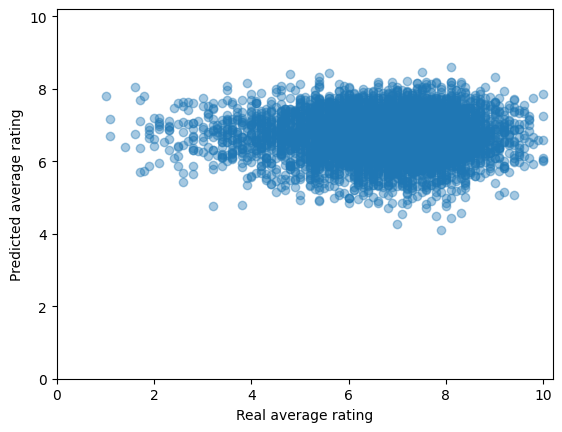
\includegraphics[width=\columnwidth]{../results/images/knn_regression_rating.png}
    \caption{Relationship between real and predicted values of average rating (KNN regressor).}
    \label{fig:knn_regression_rating}
\end{figure}

\begin{figure}
    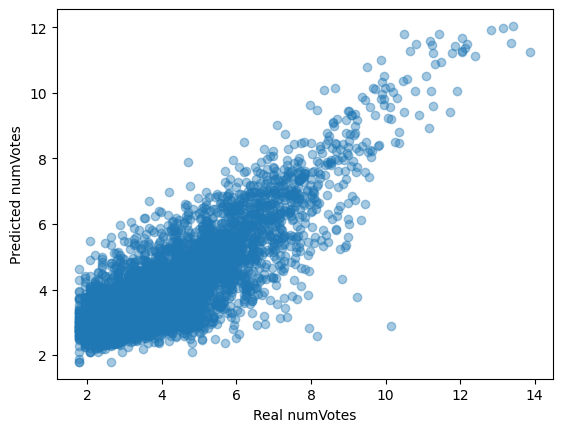
\includegraphics[width=\columnwidth]{../results/images/knn_regression_votes.png}
    \label{fig:knn_regression_votes.png}
\end{figure}

\subsection{Decision Tree Regressor}
We trained the DT regressor on all (categorical and numerical) features with the same preprocessing described for classification.
In order to determine the best combination of parameters, we performed random search on the same hyperparameter space defined for the classification task (except we used only MSE as splitting criterion).

For the \textbf{average rating}, we fitted and tested a DT regressor with the following parameters:
\begin{itemize}
    \item max\_depth: 2
    \item min\_samples\_split: 2
    \item min\_samples\_leaf: 100
\end{itemize}
Again, the model performace proved unsatisfactory, with a \textbf{R2 score} of \textbf{0} and a \textbf{MSE} of \textbf{1.83}.

For the \textbf{number of votes}, we fitted and tested a DT regressor with the following parameters:
\begin{itemize}
    \item max\_depth: 11
    \item min\_samples\_split: 50
    \item min\_samples\_leaf: 15
\end{itemize}
which performed slightly worse than the KNN regressor:
\textbf{R2: .67}, \textbf{MSE: 1}.
We inspected the features with higher feature importance (calculated as total reduction in negative MSE brought by each feature) in order to determine which numerical features we should attempt to use for the linear regression.
According to the model the three top features were \emph{criticReviewsRatio}, \emph{numRegions} and \emph{totalCredits}.

\subsection{Linear models}

Since none of our numerical features showed any correlation with the mean rating, we attempted to fit an ordinary least squares linear regressor using all numeric variables as input.
This model obtained a \textbf{R2 score} of \textbf{0} and a \textbf{MSE} of \textbf{1.83}.

For \textbf{numVotes}, we performed model selection among models using different combinations of input variables and regularization (since some of our input variables are correlated with each other, we used Ridge regularization).

We used the following combinations of features:
\begin{enumerate}
    \item Top 3 DT features: \emph{criticReviewsRatio}, \emph{numRegions}, \emph{totalCredits};
    \item Top 3 correlated features: \emph{totalImages}, \emph{numRegions}, \emph{totalCredits};
    \item all numerical features.
\end{enumerate}
For each combination of input variables we performed 5-fold cross validation on the training set with and ordinary least squares linear regressor and reported the R2 score.

For the Ridge regressor, we used the leave-one-out cross-validation built in sklearn \texttt{RidgeCV} in order to determine the best value of $\alpha$ (checking for powers of 10 between 10\textsuperscript{-3} and 100), in all cases we found that the best $\alpha$ was 10.

\begin{table}
    \begin{tabular}{lrr}
        \toprule
        Feature combination & OLS & Ridge\\
        \midrule
        top DT & 0.459 & 0.459 ($\alpha=10$)\\
        top correlated & 0.518 & 0.519 ($\alpha=10$)\\
        all & 0.547 & 0.548 ($\alpha=10$) \\
        \bottomrule
    \end{tabular}
    \caption{Validation R2 scores for all linear regressors.}
    \label{tab:linear_regression_validation}
\end{table}

Table \ref{tab:linear_regression_validation} reports the scores obtained in validation: we can see that applying regularization had little effect on the performance of our models and that the best performing model uses all numerical features in input and Ridge regularization with $\alpha$=10.

We then tested the best model, obtaining a \textbf{R2 score} of \textbf{0.55} and a \textbf{MSE} of \textbf{1.389}.

\subsubsection{Conclusions}
We were not able to fit any regressor that could predict the average rating of a title adequately.

On the other hand, when using \emph{numVotes} as target variable we were able to obtain good results.
As evidenced by the reported scores, non-linear models performed much better than linear ones because they were able to model non linear relationships between the input variables and the target.

KNN performed slightly better than DT.
Considering that this slight improvement comes at the cost of less interpretable results and greater computational cost at prediction time, it could be argued that DT is still the better model.
On the other hand DT also uses more features and KNN can be adapted to new data without retraining the model, so the preference for one model over the other may very well depend on the specific application.